\chapter*{Ray-Marching}

${ }$\\
$\textbf{MÍO}$
${ }$\\

En Ray-Marching para calcular las intersecciones de los rayos con una superficie dada en su ecuación implícita, la cual es de la forma
\[
	F(x,y,z) = 0,
\]
vamos a usar dos métodos de aproximación de soluciones que son Newton-Raphson y Regula-Falsi. cada uno tiene unas ventajas e inconvenientes que justifican el uso de ambos de forma combinada. El primero de ellos no garantiza que se llegue a una aproximación de la solución ya que la sucesión que genera puede divergir como se verá mas adelante, pero este método converge mas rápido que el segundo. Para comprobar este hecho introduciremos algunos términos como el orden de convergencia. 


${ }$\\
$\textbf{Newton-Raphson}$
${ }$\\

\begin{figure}
	\begin{center}
		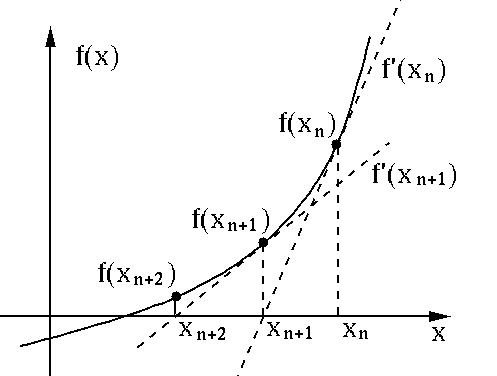
\includegraphics[width=0.8\textwidth]{imagenes/newton.png}
	\end{center}
	\caption{Construcción gráfica de la sucesión dada por el método de Newton-Raphson}
	\label{fig:etiq_7}
\end{figure}

Como se puede ver en la Figura \ref{fig:etiq_7} el método de Newton-Raphson comienza con un valor $x_0$ que es una primera aproximación, y para calcular el siguiente valor de la sucesión toma la pendiente de la función en el punto $(x_0, f(x_0))$, entonces $x_1$ será la intersección del eje de abscisas con la recta tangente que acabamos de ver.
${ }$\\

El algoritmo a seguir es el siguiente:

\begin{itemize}
	\item Paso 0 : Tomar un $x_0$ inicial.
	\item Paso 1 : $x_{n+1} = x_n - \frac{f(x_n)}{f'(x_n)}$.
\end{itemize}

Se puede observar que no siempre es posible calcular el siguiente $x_n$ ya que la derivada de la función en $x_{n-1}$ podría ser $0$.
${ }$\\
${ }$\\

${ }$\\
$\textbf{Regula-Falsi}$
${ }$\\

El algoritmo de Regula-Falsi es un refinamiento de el método de bisección. Al igual que en el método de bisección partimos de un intervalo inicial $[a_0, b_0]$, teniendo $f(a_0)$ y $f(b_0)$ signos opuestos, ya que como dice el Teorema\ref{teo:bolzano} esto nos garantiza que hay una solución dentro de ese intervalo, aunque por el procedimiento que sigue este algoritmo es posible no encontrar soluciones que correspondan con un mínimo o un máximo de la función. Este método va calculando intervalos cada vez mas pequeños que incluyen a la solución.
${ }$\\

Como se puede ver en la Figura \ref{fig:etiq_8}, gráficamente el procedimiento toma la recta que pasa por los puntos $(a_0, f(a_0))$ y $(b_0, f(b_0))$ y toma el punto de intersección de esta con el eje de abscisas el nuevo intervalo se ajustará dependiendo de que el valor de la función en este nuevo punto sea negativo a positivo, $f(a_1) \cdot f(b_1) < 0$.

\begin{teorema}\label{teo:bolzano}
	$\textbf{(de los ceros de Bolzano)}$ Sea una función continua $f : [a,b] \to \mathbb{R}$ tal que $f(a) \cdot f(b) < 0$, entonces existe al menos un $s \in (a,b)$ tal que $f(s) = 0$.
\end{teorema}



El algoritmo de Regula-Falsi es el siguiente:

\begin{itemize}
	\item Paso 0 : Tomar un $a_0$ y $b_0$ iniciales.
	\item Paso 1 : $m_n = \frac{a_n f(b_n) - b_n f(a_n)}{f(b_n) - f(a_n)}$
	\begin{itemize}
		\item Si $f(m_n)=0$, hemos terminado.
		\item Si $f(a_n) \cdot f(m_n) < 0$, $b_n = m_n$.
		\item Si $f(b_n) \cdot f(m_n) < 0$, $a_n = m_n$.
	\end{itemize}
\end{itemize}

\begin{figure}
	\begin{center}
		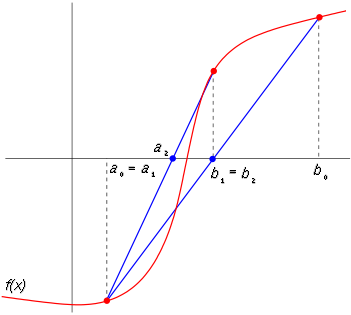
\includegraphics[width=0.8\textwidth]{imagenes/regulaF.png}
	\end{center}
	\caption{Construcción gráfica del método de Regula-Falsi}
	\label{fig:etiq_8}
\end{figure}




${ }$\\
$\textbf{Comparación de métodos}$
${ }$\\


\begin{definicion}
	Sea $p \in \mathbb{R}$ y $p > 1$. Diremos que la sucesión $\{ x^{(k)} \}^{\infty}_{k=1}$ convergente a $s$ de números reales \underline{\textbf{converge}} a $s$ \underline{\textbf{con al menos orden de convergencia $p$}} si $|x^{(k)} -s| \leq \epsilon_k$, $\forall k = 1,2,3...$, siendo $\{ \epsilon_k \}^{\infty}_{k=1}$ una sucesión de números reales positivos tal que
	\[
		\lim_{k \to \infty} \frac{\epsilon_{k+1}}{\epsilon^{p}_{k}} = C
	\]
	con $C > 0$ si $p > 1$, y $0 < C < 1$ si $p = 1$.
	${ }$\\
	
	Por otro lado, si $\epsilon_k = |x^{(k)} -s|$, $\forall k = 1,2,3...$, entonces diremos que la sucesión converge a s con orden de convergencia $p$ y constante asintótica del error igual a $C$.
	\begin{itemize}
		\item Si $p=1$,llamamos lineal al orden de convergencia.
		\item Si $p=2$, la llamamos cuadrática.
	\end{itemize}
\end{definicion}

Hay que tener en cuenta que para mayores valores de $p$ mayor es la rapidez con que converge.
${ }$\\

Para el caso de Newton-Raphson encontramos dos resultados que nos indican cuales son los ordenes de convergencia que nos podemos encontrar a la hora de aplicar ese método. Uno de ellos es para una función cuyo cero queremos encontrar es simple, es decir, $f'(s) \neq 0$ para $s$ raíz de $f$; y el otro para el caso de que la raíz sea un cero múltiple.

\begin{definicion}
	Sea $f \in C^M([a,b])$ y $s$ valor donde $f$ se hace cero, diremos que es de multiplicidad $M$ si y sólo si $f^{(k)}(s) = 0$, $k = 0, ..., M-1$ y $f^{(M)}(s) \neq 0$. Si $M = 1$ se llama cero simple.
\end{definicion}

\begin{teorema}
	Sea $f \in C^2(U_S)$ con $U_S$ un entorno de $s$ tal que $f(s) = 0$ y $f'(s) \neq 0$. Entonces, $\exists \epsilon > 0$ tal que si $|x^{(0)} - s| \leq \epsilon$ la sucesión generada por el método de Newton-Raphson converge a $s$ con convergencia cuadrática y constante asintótica del error $\frac{|f''(s)|}{2|f'(s)|}$.
\end{teorema}

\begin{proof}
	${ }$\\
	
	En lo que sigue consideraremos el desarrollo en serie de Taylor
	\[
		f(x) = f(x_n) + (x - x_n)f'(x_n) + \frac{(x - x_n)^2}{2} f''(\xi)
	\]
	siendo $\xi$ un punto intermedio entre $x$ y $x_n$. Si $x=s$, $s$ una raíz de $f$ y dividiendo por $f'(x_n)$, obtenemos
	\[
		s = x_n - \frac{f(x_n)}{f'(x_n)} - \frac{(s - x_n)^2}{2} \cdot \frac{f''(\xi_n)}{f'(x_n)}
	\]
	siendo $\xi_n$ un punto intermedio entre $s$ y $x_n$. Finalmente usando la expresión del método de Newton-Raphson, tenemos
	\[
		s - x_{n+1} = - (s - x_n)^2 \cdot \frac{2f''(\xi_n)}{f'(x_n)}
	\]
	
	Como $f'(s) \neq 0$ y $f'$ es continua en $U_S$, entonces $\exists \delta > 0$ tal que $f'(x) \neq 0$ $\forall x \in I_{\delta} = [s - \delta, s + \delta]$. Ahora consideremos
	\[
		M = M(\delta) = \frac{\max_{x \in I_{\delta}} |f''(x)|}{2 \min_{x \in I_{\delta}} |f'(x)|}.
	\]

	Por tanto, podemos llegar a que
	\[_
		|s - x_1| \leq M |s - x_0|^2
	\]
	\[_
		M|s - x_1| \leq (M |s - x_0|)^2
	\]
	de donde podemos fácilmente deducir por inducción que
	\[
		|s - x_n| \leq \frac{1}{M} (M |s - x_0|)^{2^n}
	\]
	
	Para terminar de probar la convergencia comprobaremos que existe un $\epsilon > 0$ con $\epsilon < \delta$ tal que $\epsilon M(\epsilon) < 1$. Así que veamos que siempre es posible encontrar dicho $\epsilon$.
	
	\begin{itemize}
		\item Si $\delta M(\delta) < 1$, entonces $\epsilon = \delta$.
		\item Si $\delta M(\delta) \geq 1$, entonces $\epsilon = \delta_1$ donde $0 < \delta_1 < \delta$ y $\delta_1 M(\delta_1) < 1$. Esto posible ya que si
		
		\[
			\delta_1 < \delta \Rightarrow I_{\delta_1} \subset I_{\delta} \Rightarrow
		\]
		\[
			\max_{x \in I_{\delta_1}} |f''(x)| \leq \max_{x \in I_{\delta}} |f''(x)| \;\;\;\; y \;\;\;\; \min_{x \in I_{\delta_1}}|f'(x)| \geq \min_{x \in I_{\delta}}|f'(x)|
		\]
		\[
			\Rightarrow M(\delta_1) \leq M(\delta)
		\]
	\end{itemize}
	
	Por tanto podemos encontrar un $\delta$ tal que $\delta M(\delta) < 1$, es decir, ya que $x_0 \in I_{\delta}$, tenemos $M(\delta)|s - x_0| < 1$. Entonces,
	\[
		|s - x_n| \leq \frac{1}{M} (M |s - x_0|)^{2^n}
	\]
	nos dice que $x_n$ converge a $s$.
	
	Dicho esto, como $\xi_n$ se encuentra entre $s$ y $x_n$ entonces $\xi_n$ tiende a $s$ cuando $n$ tiende a $\infty$. Y por tanto,
	\[
		\lim_{n \rightarrow \infty} \frac{|s - x_{n+1}|}{|s - x_{n}|^2} = - \lim_{n \rightarrow \infty} \frac{f''(\xi_n)}{2f'(x_n)} = - \frac{f''(s)}{2f'(s)}.
	\]
\end{proof}

\begin{teorema}
	Sea $f \in C^2(U_S)$ con $U_S$ un entorno de $s$ tal que $f(s) = 0$. Entonces, el método de Regula-Falsi converge a $s$ con orden de convergencia lineal y constante asintótica del error $(\frac{|f''(s)|}{2|f'(s)|})^{(\varphi - 1)}$.
	
\end{teorema}

\begin{proof}
	Para cada iteración $n$ de Regula-Falsi calculamos la ecuación de la recta que pasa por los puntos $(a_n, f(a_n))$ y $(b_n, f(b_n))$
	\[
		y - f(b_n) = \frac{f(b_n) - f(a_n)}{b_n - a_n}(x - b_n),
	\]
	ahora haciendo $y = 0$ obtenemos la fórmula vista para el algoritmo
	\[
		m_n = b_n - f(b_n) \frac{b_n - a_n}{f(b_n) - f(a_n)} = \frac{a_n f(b_n) - b_n f(a_n)}{f(b_n) - f(a_n)}
	\]
	
	Vamos a representar el error en la n-ésima iteración por $e_n = m_n - s$ y para demostrar que la convergencia es lineal usaremos la siguiente expresión obtenida de restar $s$ a la expresión anterior
	\[
		m_n - s = b_n - s - f(b_n) \frac{b_n - a_n}{f(b_n) - f(a_n)}
	\]
	
	También haremos uso del desarrollo en serie de Taylor para aproximar la función $f$
	\[
		f(x) = f(s) + (x - s) f'(s) + \frac{(x - s)^2}{2} f''(s)
	\]
	donde sabemos que $f(s) = 0$ y por tanto para $a_n$, $b_n$
	\[
		f(a_n) = (a_n - s) f'(s) + \frac{(a_n - s)^2}{2} f''(s)
	\]
	\[
		f(b_n) = (b_n - s) f'(s) + \frac{(b_n - s)^2}{2} f''(s).
	\]
	Calculamos
	\[
		f(b_n) - f(a_n) = f'(s) (b_n - a_n) + \frac{f''(s)}{2}[(b_n - s)^2 - (a_n - s)^2]
	\]
	\[
		= (b_n - a_n) [f'(s) + \frac{f''(s)}{2} (b_n + a_n - 2p)],
	\]
	con esto y $f(b_n)$ podemos obtener
	\[
		m_n - s = (b_n - p)[1 - \frac{f'(s) + \frac{f''(s)}{2} (b_n - s)}{f'(s) + \frac{f''(s)}{2} (b_n + a_n - 2p)}]
	\]
	\[
		= (b_n - p) (a_n - p) \frac{f''(s)}{2 f'(s) + f''(s) (b_n + a_n - 2p)}
	\]
	
	Tengamos en consideración que llega un momento en el que el intervalo es tan pequeño que el signo de su derivada y segunda derivada se conserva, supongamos que esto ocurre en una iteración $i$. Entonces, sin perdida de generalidad supondremos que $f'(x) \geq 0$ y $f''(x) \geq 0$ para $x \in [a_i, b_i]$. Llegados a este punto, por la forma que toma la función habrá un extremo del intervalo que quedará fijo para $n \geq i$. A partir de esto y considerando que $e_{n-1} = m_{n-1} - s = b_n - s$
	
	\[
		e_n = e_{n-1} (a_n - s) \frac{f''(s)}{2 f'(s) + f''(s) (e_{n-1} + a_n - p)}
	\]
	
	Definiendo
	\[
		\lambda \simeq \frac{l f''(s)}{2 f'(s) l f''(s)},
	\]
	donde $l = (a_n - s)$ cuando $a_n$ queda fijo y $l = (b_n - s)$ cuando $b_n$ queda fijo, podemos concluir que
	\[
		e_n \simeq \lambda e_{n-1}
	\]
	
	Por tanto la sucesión de Regula-Falsi converge con orden de convergencia lineal.
\end{proof}


${ }$\\
$\textbf{Criterio de parada}$
${ }$\\

El algoritmo que queremos implementar va calculando los elementos de una sucesión que converge a la solución pero en la mayoría de los casos no llega a ser la solución exacta y hay infinitos términos de la sucesión por lo que tenemos que elegir un método que nos diga cuando queremos que pare de calcular elementos de la sucesión. Usaremos como método uno de los siguientes criterios de parada: para cuando se hayan realizado un número determinado de iteraciones, parar cuando $|f(x_n)| < \epsilon$, parar cuando $|x_{n-1} -x_n| < \epsilon$ donde $\epsilon > 0$. En este caso vamos a usar que $|f(x_n)| < \epsilon$.


${ }$\\
$\textbf{INTRODUCCIÓN}$
${ }$\\

Las ecuaciones implícitas de superficies son de la forma $F(x, y, z) = 0$ esta forma es adecuada para imágenes con sombreado. Las coordenadas de pixeles son sustituidas por $x$ e $y$ y la ecuación es resuelta para z. Los algoritmos para dibujar tales objetos se han desarrollado principalmente para funciones polinomiales de primer y segundo orden, una subcategoría conocida como superficies algebraicas. Este artículo presenta un nuevo algoritmo aplicable a otras formas funcionales, en particular a la suma de varias distribuciones de densidad gaussianas. El algoritmo fue creado para modelar mapas de densidad electrónica de estructuras moleculares, pero puede ser utilizado para otras formas artísticamente interesantes.

La tecnología de crear imágenes realistas y visualmente interesantes de tres
las formas dimensionales están avanzando en muchos frentes. Uno de ellos es el desarrollo de algoritmos para dibujar superficies curvas directamente desde sus definiciones matemáticas en lugar de dividirlas en grandes cantidades de polígonos. Dos clases de superficies que han recibido atención son las superficies paramétricas cuádruples y las bivariadas. Las superficies paramétricas bivariadas se generan mediante tres funciones de dos variables (la mayoría de las veces son polinomios), ya que las variables adquieren diferentes valores.

Superficies cuádricas, por otro lado, son soluciones de ecuaciones de segundo orden.

\[
	ax^2 + bxy + cxz +dx +ey^2 +fyz +gy + hz^2 + iz +j = 0.
\]

Esta clase de superficies incluye formas tales como esferas, conos o hiperboloides de revolución. Como podemos ver las cuadricas son soluciones de ecuaciones implicitas que como hemos dicho son de la forma $F(x, y, z) = 0$.

Este documento examina una solución más general al problema de imágenes para tales superficies y describe en detalle su aplicación a una clase de superficies que están estrechamente relacionadas con los cuadrículas pero que tienen una gama más amplia de formas.


${ }$\\
$\textbf{EL MODELO}$
${ }$\\

El problema que motivó este documento es el familiar en los gráficos por computadora de mostrar modelos moleculares. Esto se hace con mayor frecuencia con un modelo de bola y bastón o un modelo de esfera llenadora de espacio. En cualquier caso, el modelo consiste en una colección posiblemente interseccionada de dos formas básicas: esferas y cilindros. Para dibujar una imagen del modelo, las esferas y los cilindros se pueden dividir fácilmente en polígonos y pasar a un algoritmo convencional de representación de polígonos. Alternativamente, se puede emplear cualquiera de varios algoritmos de superficie curva, y, de hecho, se han formulado varios algoritmos de propósito especial [6, 8, 9] para manejar eficientemente solo estas dos formas para la visualización rápida de estructuras moleculares grandes.

En interés tanto de la variedad artística como de la precisión científica, se buscó un nuevo modelo que se separe del molde de bola y adhesivo / relleno de espacio. Se deseaba hacer que los enlaces entre los átomos se parecieran más a los que se muestran en la Figura 1. Esto es, de hecho, más parecido a lo que podría parecer una nube de densidad de electrones real para un enlace covalente. Además, a los efectos de la animación, este vínculo debe estirarse y contraerse de una manera agradable, ya que vibra, rompiendo a medida que un átomo se aleja por completo de la molécula. Esto se ilustra en la Figura 2.

Un enfoque convencional podría ser modelar dicha forma a través de las superficies bicúbicas o cuádricas ya familiares. Esto es moderadamente factible para un enlace aislado pero se vuelve difícil para moléculas más elaboradas con varios enlaces superpuestos (por ejemplo, estructuras de anillo). Además, los cambios topológicos que deben ocurrir cuando se rompe un enlace son difíciles de manejar de manera automatizada. Por estas razones, se utilizó un modelo matemático básico que es similar en forma a una simulación real de mapas de densidad de electrones. La mecánica cuántica representa el electrón en un átomo como una función de densidad de la ubicación espacial. Una función de muestra para un átomo de hidrógeno es

\[
	D(x, y, z) = exp(-ar)
\]
donde $r = \sqrt{(x-x_1)^2 + (y-y_1)^2 + (z-z_1)^2}$ y $(x_1, y_1, z_1)$ la localización del átomo.

Podemos representar esta función para una colección de átomos sumando la contribución de cada átomo por separado.
\[
	D(x, y, z) = \sum_{i} b_i exp(-a_i r_i)
\]
donde $r_i$ es la distancia de $(x,y,z)$ al centro del átomo $i$.

Una superficie se puede definir como aquellos puntos donde esta función de densidad es igual a una cantidad umbral:
\[
	F ( x, y, z) = D ( x, y, z) - T.
\]

Tenga en cuenta que todos los puntos dentro de la superficie tienen densidades de electrones mayores que T. A los efectos de la eficiencia computacional, la función realmente implementada fue de forma similar:
\[
	D(x, y, z) = \sum_{i} b_i exp(-a_i r^{2}_{i})
\]
Esto no requiere tomar una raíz cuadrada. El término exponencial es simple
Golpe gaussiano centrado en ri, con altura bi y desviación estándar ai. Ajustando los parámetros ai y bi, se pueden lograr diferentes efectos para la misma disposición de átomos. Estos efectos alteran el "blobbiness" del objeto. De hecho, para fines de modelado, es más útil para un diseñador especificar estos dos parámetros en términos del radio del átomo en aislamiento y un parámetro de blobbiness. El radio de un átomo aislado Ri se encuentra al establecer
\[
	T = b_i exp(-a_i R^{2}_{i}) = exp (-a_i R^{2}_{i} + ln (b_i))
\]
entonces el ai puede ser elegido para ser
\[
	a_i = - \frac{ln(T/b_i)}{R^{2}_{i}}
\]
Podemos definir el parámetro blobbiness para ser
\[
	B_i = ln(T/b_i)
\]
de modo que (resolviendo para bi)
\[
	b_i = T exp(-B_i)
\]
La contribución de densidad neta de un átomo en términos de los dos parámetros que definen la forma Ri y Bi es
\[
	D_i(x,y,z) = T \; exp ( \frac{B_i}{R^{2}_{i}}r^{2}_{i} -B_i)
\]
Tenga en cuenta que Bi debe ser negativo para garantizar que la función de densidad vaya a cero a medida que ri va al infinito.

Como hay un factor de T en cada átomo contribuyente, el valor del umbral ahora es irrelevante; podemos establecerlo en algún valor canónico como 1. Uno puede obtener el mismo efecto que cambiar el umbral ajustando los factores de escala, bi, de los términos individuales (es decir, ajustando los parámetros de blobbiness Bi). Sin embargo, para mayor claridad, generalmente escribimos el umbral como T, en el entendimiento de que T = 1. Un valor de umbral canónico de 1 es particularmente conveniente ya que su logaritmo es 0. La superficie definida por un átomo aislado, definida por el ajuste Di = T, es entonces una superficie cuádrica convencional. Esto se ve tomando el logaritmo de ambos lados de la ecuación anterior, produciendo 0 = (Bi / R2i) r2i - Bi. En la Figura 3 se muestra una imagen de muestra que muestra un rango de tales parámetros.

${ }$\\
$\textbf{EL ALGORITMO DE RENDERIZADO}$
${ }$\\

Las superficies definidas algebraicamente son intrínsecamente adecuadas para los algoritmos de conversión de trama. La estructura general de dicho algoritmo es sencilla: para cada ubicación de píxeles (xs, ys) la ecuación algebraica de definición se reduce a una ecuación univariante en z. Las soluciones a esta ecuación (si las hay) producen la profundidad z de la superficie en ese píxel. En el caso de las superficies cuádricas más comunes, esta solución es fácil de obtener. En el caso de las superficies más generales que se describen aquí, la solución debe obtenerse numéricamente. La parte importante del algoritmo descrito aquí es una técnica para acelerar este cálculo.

${ }$\\
$\textbf{Algoritmo básico}$
${ }$\\

Para un píxel particular, el cuadrado de la distancia desde el centro del átomo i, Pi, a un punto en el rayo de visión, $z \overline{R}$, se reduce a un polinomio cuadrático en z.
\[
	r^{2}_{i} = (z\overline{R} - \overline{P}_i)\cdot(z\overline{R} - \overline{P}_i) = z^2(\overline{R} \cdot \overline{R}) - 2 z (\overline{R} \cdot \overline{P}_i) + (\overline{P}_i \cdot \overline{P}_i)
\]
Esta expresión es algebraicamente correcta, pero desafortunadamente es susceptible de un error de redondeo. La razón para esto se puede ver en la Figura 4.

La función puede ser una parábola bastante estrecha centrada posiblemente bastante atrás en el eje z. Si bien los valores comúnmente encontrados para los coeficientes de esta ecuación no presentan por sí mismos problemas, la solución de la ecuación requiere tomar diferencias de sus productos. Esto puede exceder fácilmente la precisión de la aritmética de precisión simple. Para evitar la necesidad de una aritmética de precisión múltiple, adoptamos una representación más geométricamente significativa
\[
	r^{2}_{i} = (\overline{R} \cdot \overline{R})(z - z^{2}_{mi}) + M_i
\]
donde
\[
	z_{mi} = (\overline{R} \cdot \overline{P}_i)/(\overline{R} \cdot \overline{R}) \;\;\;\;\;\; y \;\;\;\;\;\; M_i = (z_{mi} \overline{R} - \overline{P}_i) \cdot (z_{mi} \overline{R} - \overline{P}_i)
\]
Aquí, zmi es la distancia z del mínimo local, Mi, de ri. Cada término en la función de densidad es, por lo tanto, una función de bache gaussiana de z centrada en zmi ,. La función total es la suma de varios de estos golpes. El valor de profundidad z visible es la primera ubicación donde esta función excede el valor T. Esto se muestra en la Figura 5.

Si solo se ve un átomo, la profundidad z se puede encontrar analíticamente estableciendo el término de densidad para ese átomo igual al valor umbral de 1.
\[
	T = 1 = exp ( -a_i r^{2}_{i} - B_i)
\]
Tomando el logaritmo de ambos lados y sustituyendo nuestra fórmula por r2i,
\[
	0 = a_i [(\overline{R} \cdot \overline{R})(z-z^{2}_{mi}) + M_i] + B_i.
\]
Resolviendo z (nótese que la raíz cuadrada negativa se toma para obtener la solución más cercana al ojo),
\[
	z = z_{im} - \sqrt{\frac{a_i M_i + B_i}{-a_i (\overline{R} \cdot \overline{R})}}.
\]

${ }$\\
$\textbf{Solución iterativa}$
${ }$\\

Si hay más de un átomo, una solución analítica no es factible y debemos recurrir a métodos numéricos. Dos métodos populares para la solución iterativa de tales ecuaciones son Newton iteration y "regula falsi".

La iteración de Newton funciona comenzando con una suposición inicial y refinándola al aproximar la función D con una línea recta tangente a la función en ese punto. La solución de esta ecuación lineal produce una nueva suposición, $z_new$.
\[
	z_{new} = z - \frac{D(z) - T}{D'(z)}
\]
Los derivados se obtienen fácilmente a partir de la forma funcional.
\[
	\frac{dD}{dz} = D' = \sum_{i} -2 a_i (\overline{R} \cdot \overline{R}) (z - z_{mi}) exp(-a_i r^{2}_{i} - B_i)
\]
Tenga en cuenta que este cálculo utiliza muchos cálculos en común con el cálculo de D, por lo que la evaluación de D y D 'es relativamente económica.

Regula falsi comienza con dos conjeturas iniciales que se sabe que entre corchetes la solución: Zn, donde D (zn) <T, y zf, donde D (zf)> T. Genera una nueva suposición dibujando una línea entre (z ,, D (zn)) y (zf, D (zf)) y resolver para T.
\[
	z_{new} = \frac{z_n (D(z_f) - T) - z_f ( D(z_n) - T)}{D(z_f) - D(z_n)}
\]
El valor real de $D (z_new)$ se calcula. Si $D (z_new) <T$ entonces $z_new$ reemplaza a zn. De lo contrario, reemplaza zf. Por lo tanto, el rango entre zn y zf se contrae continuamente alrededor de la solución correcta.

Si la conjetura inicial es lo suficientemente cercana a la solución real, la iteración de Newton converge rápidamente. Si no está cerca, sin embargo, divergerá. Se garantiza que Regula falsi converge pero lo hace más lentamente. Por lo tanto, hemos adoptado una solución híbrida. Un valor para $z_new$ se calcula mediante la iteración de Newton. Si este valor está fuera del rango (Zn, Zf), entonces el valor se vuelve a calcular a partir de la fórmula regula falsi. Este proceso se repite hasta que el valor de $| D (z_new) - T |$ es menor que alguna tolerancia de error t.

Para generar el primer rango inicial de suposiciones, dependemos de algunas heurísticas basadas en nuestro conocimiento de la forma funcional. Esperamos que la solución esté en o cerca de las soluciones a las protuberancias atómicas individuales (Figura 6) o al máximo local de una protuberancia si no supera el valor umbral T (Figura 7).

Por lo tanto, hacemos una lista de posibles valores iniciales de estimación z y los ordenamos en orden ascendente de z. La lista ordenada se escanea de adelante hacia atrás y, para cada elemento, se calcula el valor real de la función (es decir, la suma de todas las contribuciones de átomos). Si esto es menor que el valor umbral, se supone que el máximo local de D cerca de aquí no alcanza el umbral y se evalúa el siguiente elemento de la lista. Si excede el valor umbral, esa z se usa como el valor inicial de zf y el elemento de la lista anterior se usa como el valor inicial de zn. Ver la Figura 8.

${ }$\\
$\textbf{Cálculos de intensidad}$
${ }$\\

Cuando se encuentra una solución z, se sustituye en eq. (*) para obtener las ubicaciones xey del punto visible en la superficie en el espacio de visualización. Para calcular una intensidad, es necesario encontrar la superficie normal en este punto. Esto se puede encontrar tomando el gradiente de la función de definición de superficie, F.
\[
	N = \left[ {\begin{array}{ccc}
		\frac{\partial F}{\partial x}, & \frac{\partial F}{\partial y}, & \frac{\partial F}{\partial z} \\
		\end{array} } \right]
\]
Para la función que estamos usando aquí, esto se hace fácilmente. Por ejemplo, el componente x será
\[
	\frac{dF}{dx} = D' = \sum_{i} -2 a_i (x - x_i) exp(-a_i r^{2}_{i} - B_i)
\]
Finalmente, podemos permitir que las propiedades reflectantes de la superficie (como el color) varíen sobre la superficie mezclándolas de acuerdo con las contribuciones de cada átomo. Esto se hace tomando una suma ponderada de la propiedad superficial de cada átomo, el peso elegido como el valor de Di de ese átomo. (Recuerde que estas suman el valor umbral de 1.0.) Alternativamente, como en la facilidad de los diagramas que se muestran aquí, podemos encontrar el átomo con el valor más alto de Di en el punto visible y usar sus propiedades de superficie.

${ }$\\
$\textbf{Optimizando el algoritmo}$
${ }$\\

Para las imágenes que contienen más de unos pocos átomos (hasta 4000 en algunas de las imágenes requeridas para este proyecto), la suma de la función D sobre todos los átomos está computacionalmente fuera de la cuestión. Afortunadamente, para cualquier píxel dado, la mayoría de los átomos están lo suficientemente lejos del rayo de escaneo, por lo que su contribución a la función D es insignificante. Por lo tanto, podemos economizar considerablemente utilizando en los cálculos solo los átomos que están "cerca" del rayo de exploración. El término "cerca" tiene un significado preciso al encerrar cada átomo en una esfera definida por
\[
	D_i (x,y,z) = tT,
\]
donde el valor t es la misma tolerancia de error utilizada como criterio de convergencia. Si el rayo de escaneo se cruza con esta esfera, debe haber puntos a lo largo de ella donde la contribución a D sea lo suficientemente grande como para importar. Si, por otro lado, el rayo escaneado está separado de la esfera circundante, entonces todos los puntos en él contribuyen menos que el error introducido por las condiciones de terminación de la solución numérica. El átomo puede omitirse.

El valor de la tolerancia al error, por supuesto, determina la calidad de la imagen. Una tolerancia mayor será más rápida pero la imagen tendrá un poco de ruido agregado. La Figura 9 muestra los resultados obtenidos con diferentes valores de t. El halo alrededor de cada ejemplo indica los píxeles cubiertos por las esferas de los átomos. Los errores en la superficie comienzan a ser aparentes con t = 0.03. Aparecen inicialmente como un pliegue a través del resalte en la parte superior de la forma.

El proceso de mantener una lista de átomos "cercanos" durante la renderización es similar al de mantener una lista de polígonos potencialmente visibles en algoritmos de representación de polígonos más convencionales (o quizás, de manera más adecuada, mantener una lista de esferas visibles en un dibujo de esferas) programa).

Comenzamos con el bucle externo (y). Para inicializar el ciclo, las esferas circundantes de todos los átomos se proyectan en el espacio de la pantalla y se calculan los valores y máximos y mínimos visibles. Las matemáticas exactas para esto se dan en la siguiente sección. La lista de átomos se ordena en mínimo y, formando la lista "y-enter". Durante el ciclo de exploración y, mantenemos una lista adicional de "y activados" de todos los átomos cuya esfera envolvente incluye el plano de exploración actual. Las adiciones y eliminaciones de esta lista se realizan de forma incremental cada vez a través del ciclo. Es decir, cada vez que $y_s$ se incrementa, se examina el elemento superior en la lista y-enter. Si ahora está por encima de los nuevos $y_s$, se mueve a la lista y-active y se examina el siguiente elemento en la lista y-enter. Cuando la parte superior de la lista y-enter está debajo de los nuevos $y_s$, sabemos que todos los átomos que ingresaron se han agregado. Ahora examine la lista activa para las eliminaciones. El $y_min$ de cada átomo en la lista y-active se prueba contra los nuevos $y_s$, y si está por encima de él, el elemento se elimina. Ver la Figura 10.

Dentro del bucle $ y $ hay un bucle $ x $ que recorre la pantalla. Aquí mantenemos una lista x-active con los candidatos provenientes de la lista y-active. Esto se hace de una manera exactamente análoga al ciclo y. Para cada elemento en la lista y-active, la esfera circundante se proyecta en la pantalla y se calcula el valor x máximo y mínimo. La lista y-active se ordena en $x_ {min}$ y se convierte en la lista x-enter. Dado que la lista y-active es de hecho idéntica a la lista x-enter, siempre se mantiene ordenada en x, desde la línea de exploración hasta la línea de exploración. Todas las adiciones se combinan en la lista utilizando un tipo de intercambio. A medida que el escaneo avanza de izquierda a derecha, se examina la lista x-enter para ingresar átomos y agregarlos a la lista x-active. La lista x-active se analiza en busca de átomos que salen. Vea la Figura 11.

En este punto tenemos, para un píxel dado, una lista de todos los átomos cuya esfera circundante intersecta el rayo de escaneo actual a través de ese píxel. Esta lista representa un sacrificio significativo de la totalidad de los átomos a solo aquellos que son relevantes para el píxel actual. Sin embargo, hay un nivel más de sacrificio disponible. Esto está en la dirección z. En la Sección 3.3 describimos la técnica para encontrar un punto inicial para la solución iterativa como un escaneo de adelante hacia atrás a través de una lista ordenada en z de posibles puntos de solución. Si, antes de este zscan, calculamos los valores Zmin / Zmax de las intersecciones de las esferas circundantes con el rayo escaneado, podemos mantener una lista z-active a medida que progresa zscan. En este caso, los valores de z examinados para las pruebas de entrada / salida no son valores enteros equiespaciados como en los casos xey. En su lugar, se toman uno a la vez de la lista z potencial. Sin embargo, esto no altera el principio básico. Ver la Figura 12.

Cuando ejecutamos el ciclo de iteración, la suma del Di se tomará solo para aquellos átomos lo suficientemente cercanos a la conjetura inicial como para importar. Por ejemplo, para la imagen que contiene más de 4000 átomos (Figura 13), había como máximo 6 átomos en la lista z-activa para la iteración y usualmente mucho menos.


${ }$\\
$\textbf{Cálculo del rango en x, y, z}$
${ }$\\

En esta sección, indicamos explícitamente cómo calcular las extensiones x, y y z de la esfera circundante de un átomo. Tales esferas adjuntas están definidas, como se describe en la Sección 3.5, por la ecuación
\[
	tT = D_i = exp (-a_i r^{2}_{i} - B_i)
\]
Tomando el logaritmo (y recordando que T = 1), transformamos esto en la ecuación para una superficie cuádrica
\[
	0 = a_i r^{2}_{i} + (B_i + ln(t))
\]
Para calcular $z_ {min} / z_ {max}$ para la prueba de rango de zscan, sustituimos la expresión por r2i en términos de z:
\[
	0 = a_i [(\overline{R} \cdot \overline{R})(z-z_{mi})^2 + M_i] + (B_i + ln(t))
\]
y resolviendo para z:
\[
	z_{min} = z_{mi} - D_z \;\;\;\;\;\;\; y \;\;\;\;\;\;\; z_{min} = z_{mi} - D_z
\]
donde
\[
	D_z = \sqrt{\frac{a_i M_i + B_i + ln(t)}{-a_i(\overline{R} \cdot \overline{R})}}
\]
Habrá dos raíces en esto siempre que la expresión bajo el radical sea positiva. La curva definida al establecer esto igual a cero definirá la proyección de los contornos de la silueta de la esfera circundante en la pantalla:
\[
	a_i M_i + B_i + ln(t) = 0
\]
Sustituyendo la definición de Mi y $z_ {mi}$ podemos transformar esto en
\[
	\Delta (\overline{R} \cdot \overline{R}) - (\overline{R} \cdot \overline{P}_i)^2 = 0
\]
donde $\Delta = (\overline{P}_i \cdot \overline{P}_i) + \frac{B_i + ln(t)}{a_i}$.

Recordando que $R = (x_z, y_z, 1)$ obtenemos

\[
	\Delta (x^{2}_{z} + y^{2}_{z} + 1) - (x_z x_i + y_z y_i + z_i)^2 = 0.
\]

Ahora para una línea de escaneo particular, $y_z$ es constante. Luego tenemos una ecuación cuadrática en $x_z$ cuyas soluciones dan el rango en $x_z$ para esa línea de escaneo.
\[
	x^{2}_{z} (\Delta - x^{2}_{i}) + x_z (-2 x_i (y_z y_i + z_i)) + (\Delta (y^{2}_{z} + 1) - (y_z y_i + z_i)^2) = 0.
\]
Las soluciones a esta ecuación $(x_ {z \; min}, x_ {z \; max})$ aún se deben convertir a coordenadas de píxel $(x_ {s \; min}, x_ {s \; max})$ por referencia a eq . (*)

La ecuación anterior tendrá dos raíces en todos los valores de $ y_z $ para los cuales su discriminante es positivo. Los valores de $ y_z $ para los que este discriminante se convierte en cero, por lo tanto, arrojan el máximo y mínimo $ y_z $ para los cuales la esfera que los contiene es visible.
\[
	4 x^{2}_{i}(y_z y_i + z_i)^2 - 4(\Delta - x^{2}_{i})(\Delta (y^{2}_{z} +1) - (y_z y_i + z_i)^2 ) = 0.
\]
De nuevo, las dos soluciones para $ y_z $ de esta ecuación se deben convertir a coordenadas de píxeles mediante eq. (*)

En los casos x e y, el rango de píxeles para la esfera circundante debe intersecarse con el rango de píxeles de la pantalla. Esto significa que estamos realizando un recorte en el espacio de la pantalla. Si el rango de la esfera está completamente fuera de la pantalla, puede eliminarse por completo.

${ }$\\
$\textbf{Sincronización}$
${ }$\\

El algoritmo de renderizado, al hacer algunas formas bastante interesantes, no es terriblemente rápido. En un esfuerzo por ver dónde se gasta el tiempo dentro del algoritmo, fue instrumentado para medir el tiempo. La Tabla 1 muestra los resultados para los cálculos implicados en la generación de la Figura 14, que contiene 64 átomos. Nuevamente, el halo alrededor de la molécula representa las esferas de los átomos e indica el rango de píxeles sobre el que se realizan los cálculos.

Tenga en cuenta que aunque las rutinas $y_ {scan}$ y $x_ {scan}$ tardan bastante tiempo (ya que tienen que ocuparse de listas activas más grandes), su contribución neta al tiempo de ejecución es pequeña ya que solo se llaman una vez por imagen y una vez por línea de exploración potencialmente ocupada, respectivamente. La rutina z calc es donde se calculan los valores de $z_ {mi}$, $M_i$, etc., para todos los átomos en la lista z-active. Esto es lo que toma la mayor parte del tiempo. Parte de la razón para esto no es tanto la cantidad de veces interrumpidas en la rutina como la gran cantidad de veces que se llama. Se llama una vez para cada píxel cubierto por cualquier esfera circundante, mientras que la rutina de iteración y sombreado se llama una vez por cada píxel ocupado.

También presentamos histogramas de los tamaños de las listas activas para cada uno de los escaneos anidados. Cada contenedor del histograma cuenta el número de veces que un tamaño determinado de la lista activa se pasa a la rutina. Tenga en cuenta que, debido al proceso de eliminación selectiva, las rutinas de iteración y sombreado generalmente se llamaban con listas activas de longitud 3 o inferior. Ver la Figura 15


${ }$\\
$\textbf{Modelado jerárquico}$
${ }$\\

La implementación de este algoritmo se realizó en un PDP-11, que permite un espacio de direcciones limitado para los programas de usuario. No hay suficiente memoria de usuario para un programa que hace tanto el modelado como la representación para sistemas de átomos del tamaño deseado. En consecuencia, el proceso se divide en dos programas que se comunican a través de un archivo temporal. Este archivo es, de hecho, solo la lista y-enter ordenada en $y_{max}$ para el volumen adjunto de cada átomo. Un programa de modelado de propósito general acepta comandos que controlan los parámetros de posicionamiento y blobbiness de átomos, iluminación global, parámetros de visualización, etc. Luego escribe la lista y-enter en el archivo atemporary. El programa de renderizado luego lee en este archivo, átomo por átomo, a medida que el escaneo avanza por la pantalla. Esto libera el programa de renderizado de cualquier restricción sobre el número total de átomos visibles. Solo necesita leer un átomo antes que él en el archivo y-enter list para poder saber cuándo el próximo átomo ingresará en la lista y-active. Internamente, solo mantiene la lista y activa y, por lo tanto, tiene restricciones solo en la cantidad máxima de átomos visibles en cualquier línea de escaneo. (Esta técnica también ha sido utilizada por el autor en programas de representación de polígonos y programas de representación de parches bicúbicos, las listas en esos casos son de polígonos o parches).

Todavía hay algunos límites en la cantidad máxima de átomos que puede mantener el programa de modelado. Estos se pueden relajar insertando un módulo de clasificación separado entre el modelador y el renderizador. El modelador no necesita poder almacenar todos los átomos en una escena. Simplemente se ocupa de la interpretación de la línea de comandos, el establecimiento de parámetros y la transformación de átomos para visualizar el espacio. Escribe la lista de átomos tal como la lee de un archivo de definición de molécula. El clasificador es un pequeño programa con una gran matriz. Lee el archivo y-enter list, ordena los datos y los vuelve a escribir.

Para los propósitos del modelado de moléculas polimerizadas grandes (como ADN) se empleó un esquema de modelado jerárquico alternativo. Los polímeros están formados por una gran colección de algunos módulos básicos. Para el ADN, estos módulos son los cuatro nucleótidos y unos pocos radicales libres utilizados para simular el proceso de replicación. Cada módulo se modela como un cuerpo rígido en una posición y orientación arbitrarias. La definición de un módulo enumera sus átomos constituyentes y el radio de una esfera circundante para todo el módulo. Cuando se va a crear una imagen, los módulos se ordenan primero en un orden basado en el mínimo $ y_s $ de sus esferas adjuntas. A continuación, se realiza un escaneo en la dirección y para generar la lista completa de y-enter de átomos directamente en orden ordenado. Para cada nuevo valor de $ y_s $, se examina la lista del módulo y para ver si alguno de los módulos se ha activado. Cuando un módulo se activa, se expande en sus átomos constituyentes que luego se transforman en espacio de visualización de acuerdo con la orientación y posición del módulo. Estos átomos se agregan a un conjunto candidato y-enter. Cuando se hayan expandido todos los módulos recientemente activados, se examinará el grupo y-enter pool candidato. Cualquier átomo que haya sido realmente visible en la línea de exploración se escribe en el archivo y-enter. La ventaja de este proceso es que el grupo candidato y-enter nunca llega a ser muy grande y, por lo tanto, puede manejar grandes estructuras.

${ }$\\
$\textbf{Extensiones}$
${ }$\\

El algoritmo inicial fue ideado para una tarea de propósito especial. Examinamos aquí algunas generalizaciones simples del proceso para dar una gama más amplia de formas que se pueden modelar.

${ }$\\
$\textbf{Método 1}$
${ }$\\

Una extensión obvia de las formas definidas hasta ahora es proporcionar formas primitivas no esféricas. Recuerde que la ecuación de definición original consistía en términos

\[
	exp(-a_i r^{2}_{i} - B_i).
\]

El exponente de e es solo un cuadric de caso especial:
\[
	-a_i r^{2}_{i} - B_i = -a_i((x - x_i)^2 + (y - y_i)^2 + (z - z_i)^2) - B_i
\]
\[
	(xyz1)(-a_i)  \left( {\begin{array}{cccc}
		1 & 0 & 0 & -x_i \\
		0 & 1 & 0 & -y_i \\
		0 & 0 & 1 & -z_i \\
		-x_i & -y_i & -z_i & P\\
		\end{array} } \right) \left( {\begin{array}{cccc}
		x \\
		y \\
		z \\
		1 \\
		\end{array} } \right),
\]
donde,
\[
	P = x^{2}_{i} + y^{2}_{i} + z^{2}_{i} + \frac{B_i}{a_i}.
\]

Al permitir cuadrics generales aquí, podemos tener elipsoides, cilindros, planos, etc., como primitivas de modelado. Esto se hace comenzando con una esfera de unidad canónica en el origen definido por
\[
	0 = (xyz1) \left( {\begin{array}{cccc}
		-B_i & 0 & 0 & 0 \\
		0 & -B_i & 0 & 0 \\
		0 & 0 & -B_i & 0 \\
		0 & 0 & 0 & -B_i \\
		\end{array} } \right) \left( {\begin{array}{cccc}
		x \\
		y \\
		z \\
		1 \\
		\end{array} } \right),
\]

Esto se escala, gira y traduce a la ubicación deseada mediante las técnicas de transformación estándar para cuadrículas [1], es decir, multiplicar a la izquierda por el inverso de la matriz de transformación y a la derecha por la transposición de la inversa.

\[
	Q' = T^{-1}QT^{-1t}
\]
donde $T$ es una matriz de transformación tal que $(x' \; y' \; z' \; w) = (x \; y \; z \; w)T$.

Esta expresión se elige para preservar la relación:

\[
	if \; (x\;y\;z\;w)Q(x\;y\;z\;w)^{t} = 0
\]
\[
	then \; (x'\;y'\;z'\;w')Q(x'\;y'\;z'\;w')^{t} = 0
\]

El lector puede verificar que escalando la matriz por $ R_i $ y traduciéndola a $ (x_i, y_i, z_i) $ uno obtiene solo la formulación de caso especial que utilizamos anteriormente para las esferas puras. La generalización de la mayoría de las otras ecuaciones en la discusión anterior se puede realizar haciendo los siguientes reemplazos:
\[
	a_i(\overline{R} \cdot \overline{R}) \;\;\;\;\; \to \;\;\;\;\; \overline{R}Q'\overline{R}^t
\]
\[
	a_i(\overline{P}_i \cdot \overline{R}) \;\;\;\;\; \to \;\;\;\;\; \overline{R}Q'\overline{W}^t
\]
\[
	a_i(\overline{P}_i \cdot \overline{P}_i) \;\;\;\;\; \to \;\;\;\;\; \overline{W}Q'\overline{W}^t
\]
donde
\[
	Q' = \;\; transformed \;\; (4x4) \;\; quadric \;\; matrix
\]
\[
	W = (0\;0\;0\;1)
\]
\[
	W = (x_z\;y_z\;1\;0)
\]
Una imagen de muestra aparece en la Figura 16.

Para formas de extensión infinita, como cilindros, el cálculo de los valores máximo / mínimo en $ x_s $ o $ y_s $ puede producir un rango infinito. Esto ocurre cuando no hay soluciones para el rango que determina las ecuaciones cuadráticas de la Sección 3.6. Para manejar estas situaciones correctamente, debemos recordar que estamos resolviendo estas ecuaciones no tanto para encontrar sus ceros sino para encontrar la región donde el polinomio cuadrático es positivo (ya que su raíz cuadrada es necesaria más adelante). En el caso general, esto puede producir un tramo finito (para elipsoides), un tramo infinito (el eje de un cilindro) o dos tramos semiinfinitos (hiperboloides). Con el cuidado apropiado al examinar el polinomio, estos casos se pueden distinguir fácilmente.

${ }$\\
$\textbf{Método 2 : Volumenes negativos}$
${ }$\\

Otra extensión es permitir valores negativos para $ b_i $. Esto efectivamente da volúmenes negativos. No son visibles por sí mismos, pero cuando se colocan cerca de objetos normales hacen abolladuras. Esto se debe a que sus contribuciones de densidad se restan de la suma. Una imagen de muestra aparece en la Figura 17.

De hecho, con algunos ajustes al algoritmo, debería ser posible permitir valores complejos para el $b_i$. Esto sería útil para simulaciones moleculares ya que las funciones de onda cuántica son en realidad funciones complejas. Por lo tanto, podríamos representar orbitales antienlazantes.

${ }$\\
$\textbf{Método 3 : Hiperelipsoides}$
${ }$\\

Se puede proporcionar una forma de superficie más general al permitir exponentes que no sean 2 en los términos del exponente.

${ }$\\
$\textbf{Método 4 : Otras funciones de impacto}$
${ }$\\

La extensión final considerada aquí implica alteraciones en la función exponencial. Podemos usar cualquier forma que tenga la misma forma general. De hecho, la implementación del algoritmo aquí utiliza un procedimiento de búsqueda de tablas con interpolación para una evaluación rápida de la función exponencial. Al colocar diferentes valores en la tabla, podemos cambiar fácilmente la forma de la función de relieve. Se debe tener cuidado de no derrotar a la heurística para la selección de conjeturas iniciales para la solución numérica. Básicamente, la función debe ser igual a 1 en f (0) y aumentar monótonamente sobre el rango utilizado.

${ }$\\
$\textbf{CONCLUSIÓN}$
${ }$\\

Hemos presentado un algoritmo que simula y representa simultáneamente una clase de superficies que tienen una apariencia visual interesante y que debería resultar útil para una variedad de aplicaciones. Algunas extensiones simples de este proceso muestran la promesa de generar otras formas interesantes.

Todos los algoritmos de síntesis de imágenes de escaneo de trama deben abordar el problema de anti-aliasing (por ejemplo, muestreo de área). Los algoritmos basados en superficies algebraicas están bastante arraigados en el muestreo puntual. Esto crea problemas principalmente en los bordes de la silueta ya que el cuerpo principal de la forma de la superficie no tiene altas frecuencias para alias. No se ha intentado ningún alisado explícito en las imágenes presentadas aquí. Este sería un tema fructífero para futuras investigaciones.